% METHOD
%=============================================================================
% Light curve simulations
%   - Intro
%   - Planet injections
%   - Planet detection
%   - Optimizing cadence and observing strategy
% Results
%   - Prospects: yields and predictions
% Discussion & Conclusion
%   - Caveats and challenges
%   - Implications
%=============================================================================

% Light curve simulations - Intro
We tested the potential for finding extra-galactic planets and small stars in
this survey by simulating light curves with realistic white noise properties,
cadence and realistic intermittent time coverage from ground-based
observations.
We also used these simulations to optimize our observing strategy.

%   - Planet injections
300 Exoplanet transit signals were injected into a set of 300 simulated light
curves using the {\tt batman} code \citet{kreidburg2015}.
We generated transit signals for planets with a range of randomly generated
planet radii and orbital periods, all orbiting a Sun-like star.
The orbital periods ranged from around 8 hours to 10 days and the planet sizes
ranged from 0.75 to 3 times the radius of Jupiter.

%   - Planet detection
In order to detect the planets in our simulated data set we used the astropy
BLS algorithm currently available through the github version of astropy
\racomment{(citation)}.
This algorithm fits an upside-down tophat, or `box' function, approximating
the shape of an exoplanet transit, to a light curve over a grid of orbital
periods, transit epochs and transit durations.
It reports the log-likelihood (-$1/2\chi^2$) of the light curve data, at each
value of orbital period, transit epoch and duration.
In high signal-to-noise cases the log-likelihood is greatest at the period,
duration and epoch of the injected transit.
However, when the relative size of the planet is small compared to the white
noise in the light curve, and when its orbital period is long, the
log-likelihood may not necessary peak at the true period.
When attempting to detect planet transits in our simulated light curves, we
required that the maximum BLS log-likelihood was greater than 15 (this
threshold was established using simulated light curves with no injected
exoplanet transit).
If a light curve passed this criterion, we measured the difference between the
maximum-likelihood period and the true orbital period of the planet and, if
the difference was less than 10\% of the period we injected, we classed that
as a `successful' planet detection.
Figure \ref{fig:completeness} shows a completeness map of planet detectability
as a function of injected radius and orbital period.

\begin{figure}
  \caption{The completeness of our exoplanet transit detection pipeline as a
    function of the radius and orbital period of the planet we injected into
    simulated DEC light curves.
}
  \centering
    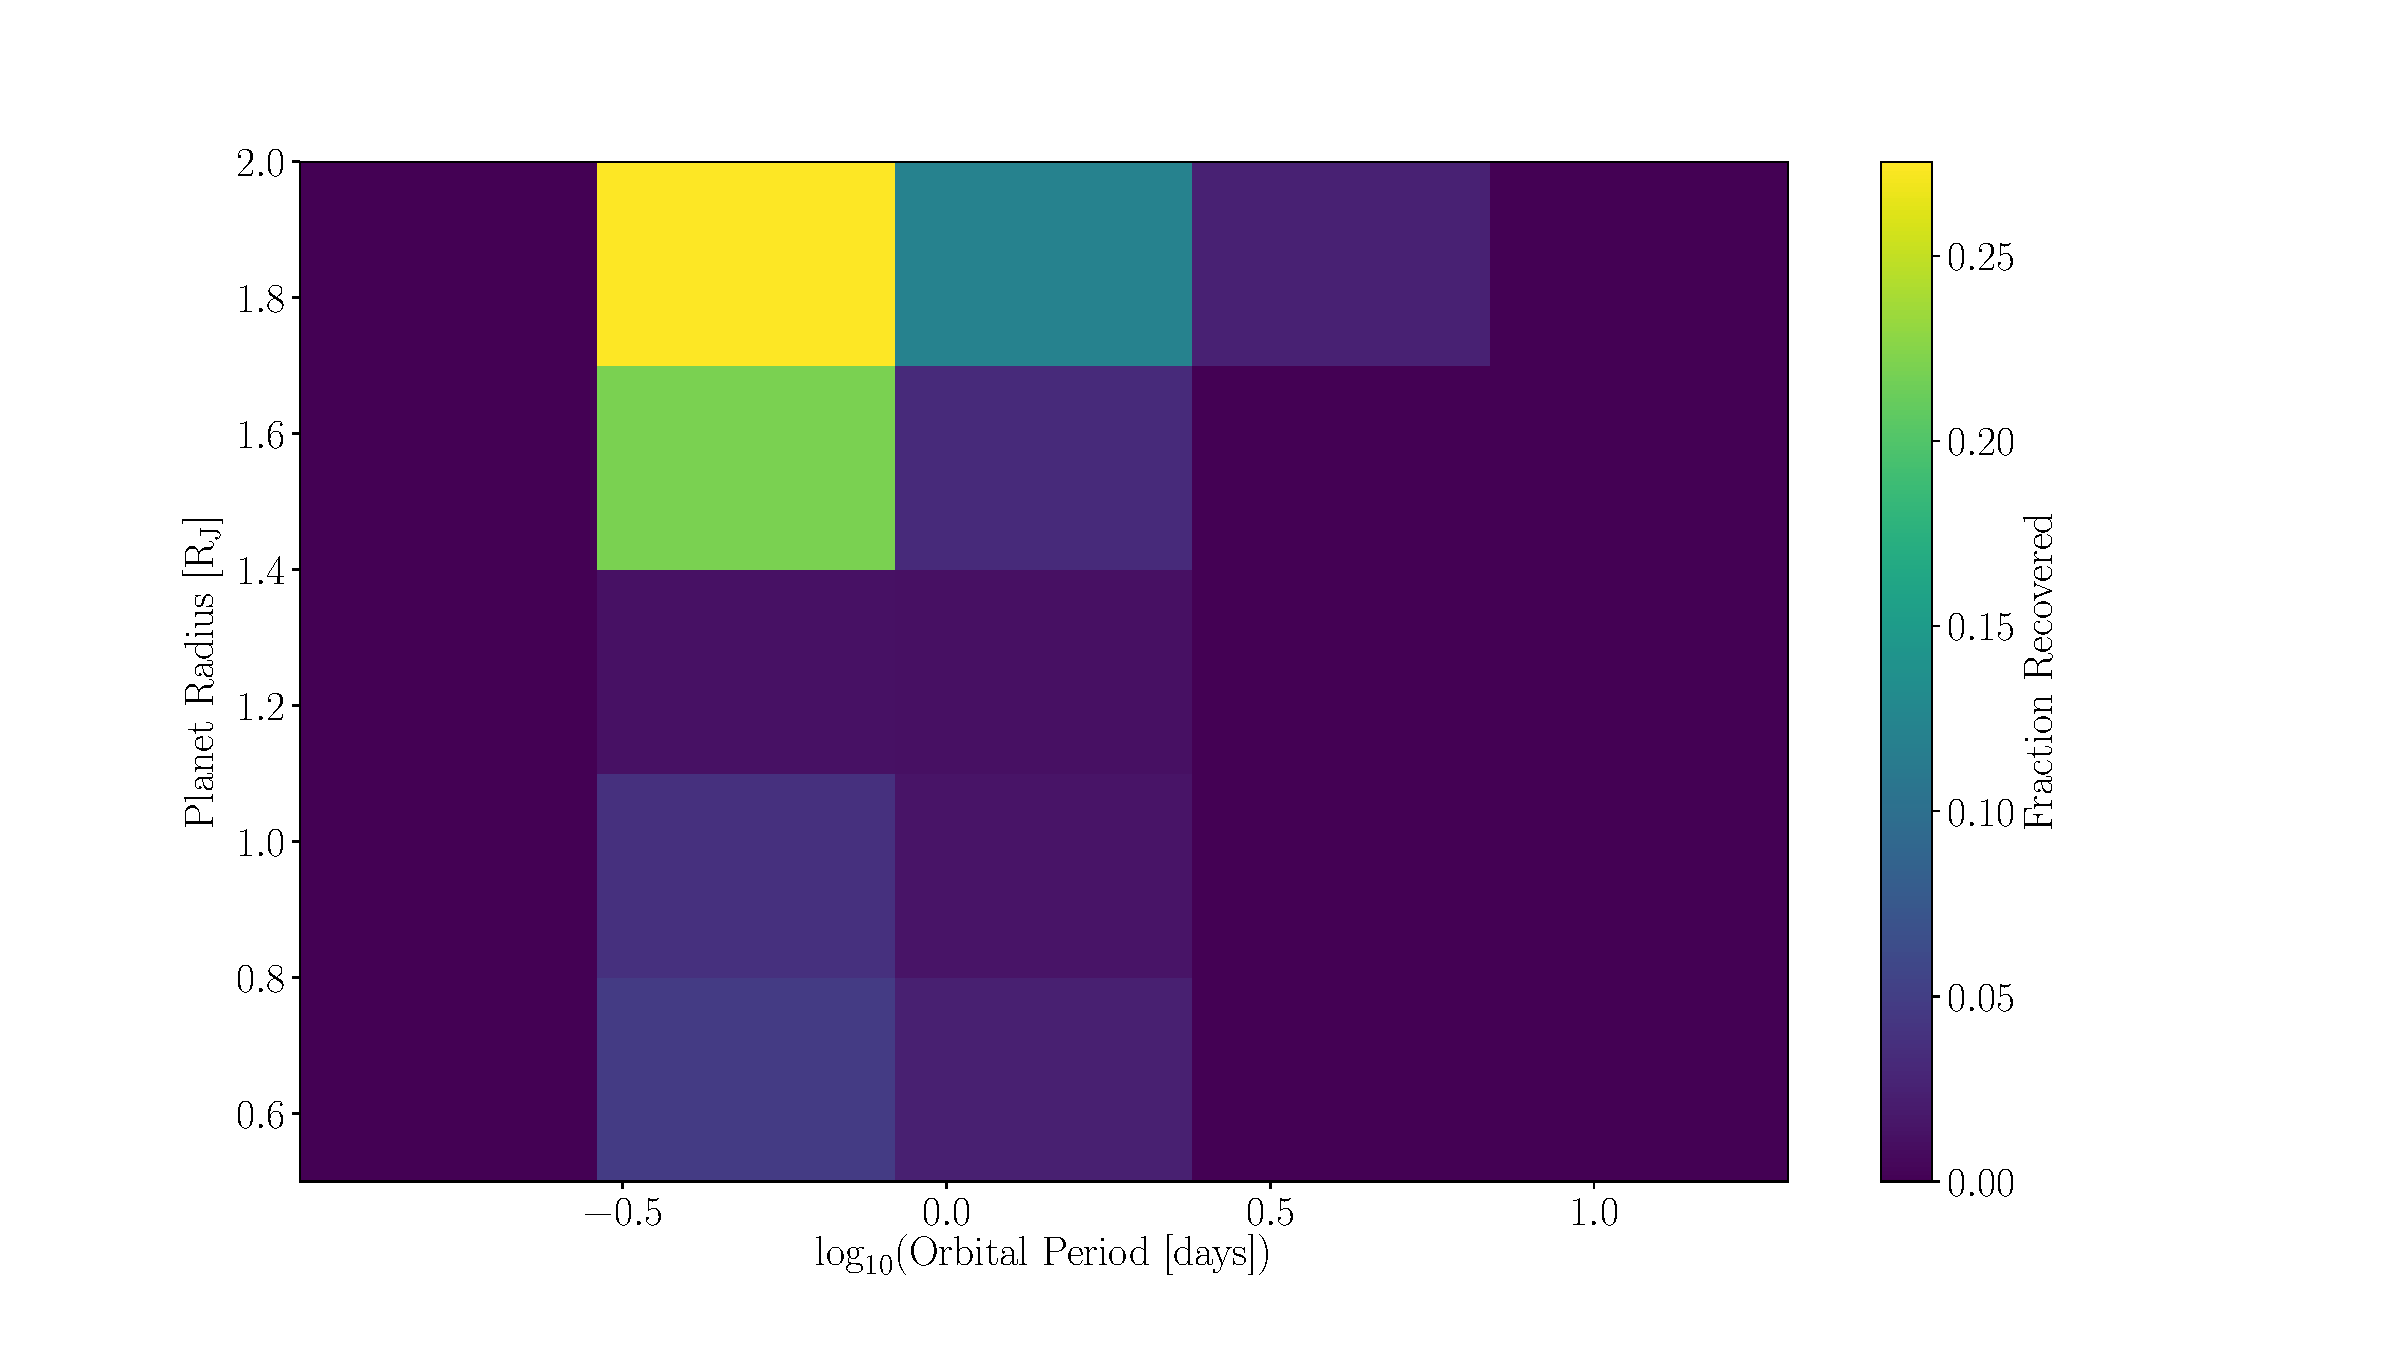
\includegraphics[width=.7\textwidth]{../completeness.pdf}
\label{fig:PGM}
\end{figure}

%   - Optimizing cadence and observing strategy
% We tested a range of cadences by injecting planets into light curves with
% different cadences and corresponding white noise amplitudes and running BLS on
% these light curves.
We simulated DEC light curves with a range of cadences and corresponding white
noise amplitudes.
We tested cadences of 3, 5, 8 and 10 minutes with SNRs of 7.0\%, 5.3\%, 4.2\%
and 3.8\% respectively and found that the most rapid cadence, 3 minute
integrations, resulted in the largest number of successfully detected
exoplanets, despite the worse photometric precision per exposure.

% Results
%   - Prospects: yields and predictions

% Discussion & Conclusion
%   - Caveats and challenges
There are several caveats to the simulations conducted here.
Firstly, we only included white noise in our simulated light curves however
time series photometry obtained from the DEC is likely to have correlated
noise due to changes in the point spread function as the instruments flex with
shifting attitude, temperature and pressure.
In addition, planet transits and eclipses may be superposed on
time-variable signals from the host star due to its rotation.
Another caveat to this study is that we only simulated transit signals with
zero impact parameter, \ie\ planets transit across the center of the star and
have the longest duration (and deepest) possible transit.

%   - Implications
These simulations indicate that we will be able to detect small stars or giant
planets orbiting Sun-like stars with Large and Small Magellanic clouds.
